

\section{Etapa 2: Implementar el comportamiento de la aplicacion }

\begin{frame}[fragile]
\frametitle{Fase 1: Crear variables para la interfaz} 
\begin{block}{MainActivity.kt}
\inputminted[linenos,fontsize=\tiny]{kotlin}{00_ComportamientoAplicacionTicTacToe/mainActivity.kt}
\end{block}

\end{frame}


\begin{frame}[fragile]
\frametitle{Concepto de Matriz}
\begin{columns}
\column{0.67\linewidth}
 
\begin{block}{Matriz}
%\inputminted[linenos,fontsize=\tiny]{kotlin}{00_ComportamientoAplicacionTicTacToe/mainActivity.kt}
\begin{itemize}
\item Colecci\'on ordenada de valores, conformada por filas y columnas
\item Los elementos pueden ser identificados por la tupla (Fila, Columna), de manera an\'aloga a un estante con fila (entepa\~no) o columna
\item Por convenci\'on, la primera fila o columna tiene el indice cero
\end{itemize}
 \end{block}

\column{0.27\linewidth}
\begin{center}
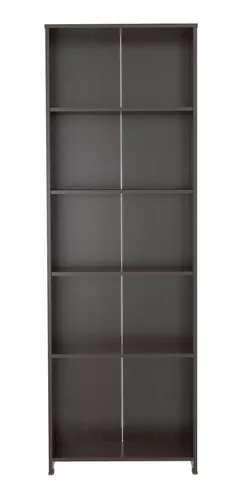
\includegraphics[width=0.95\linewidth]{00_ComportamientoAplicacionTicTacToe//Librero.png}    
\end{center}
\end{columns}


\end{frame}





\begin{frame}[fragile]
\frametitle{Fase 1: Crear variables para la interfaz} 
\begin{columns}
\column{0.47\linewidth}
\begin{block}{(*1)}
\inputminted[linenos,fontsize=\tiny]{kotlin}{00_ComportamientoAplicacionTicTacToe/imports_etapa1_fase1.kt}
\end{block}
\begin{block}{(*2)}
\inputminted[linenos,fontsize=\tiny]{kotlin}{00_ComportamientoAplicacionTicTacToe/Variables.kt}
\end{block}
\column{0.47\linewidth}
\begin{block}{(*3)}
\inputminted[linenos,fontsize=\tiny]{kotlin}{00_ComportamientoAplicacionTicTacToe/OnCreate.kt}
\end{block}

\begin{block}{(*4)}
\inputminted[linenos,fontsize=\tiny]{kotlin}{00_ComportamientoAplicacionTicTacToe/InicializarBotonesConIds.kt}
\end{block}


\end{columns}
\end{frame}



\begin{frame}[fragile]
\frametitle{Fase 1: Agregar un Listener} 
\begin{columns}
\column{0.45\linewidth}
\begin{block}{(*4)}
\inputminted[linenos,fontsize=\tiny]{kotlin}{00_ComportamientoAplicacionTicTacToe/AsignarListenerAFunciones.kt}
\end{block}

\begin{block}{(*4)}
\inputminted[linenos,fontsize=\tiny]{kotlin}{00_ComportamientoAplicacionTicTacToe/listenerVersion0.kt}
\end{block}


\column{0.45\linewidth}

\begin{block}{(*4)}
\inputminted[linenos,fontsize=\tiny]{kotlin}{00_ComportamientoAplicacionTicTacToe/CrearMatrizEstatus.kt}
\end{block}

\begin{block}{(*4)}
\inputminted[linenos,fontsize=\tiny]{kotlin}{00_ComportamientoAplicacionTicTacToe/ObtieneFilaColumna.kt}
\end{block}


\end{columns}
\end{frame}

\begin{frame}[fragile]
\frametitle{Fase 1: Reiniciar Controles a su Estado Inicial (1)} 
\begin{columns}
\column{0.48\linewidth}
\begin{block}{(*4)}
\inputminted[linenos,fontsize=\tiny]{kotlin}{00_ComportamientoAplicacionTicTacToe/ReiniciarControles.kt}
\end{block}
\column{0.48\linewidth}


\end{columns}
\end{frame}

\begin{frame}[fragile]
\frametitle{Fase 1: Agregar un Listener} 
\begin{columns}
\column{0.70\linewidth}

\begin{block}{(*5)}
\inputminted[linenos,fontsize=\tiny]{kotlin}{00_ComportamientoAplicacionTicTacToe/CeldaGato.kt}
\end{block}
\begin{itemize}
\item Hasta este punto, la aplicación responde con un mensaje en cada celda seleccionada, con el numero de fila y columna en la cual se ubica
\end{itemize}

\column{0.20\linewidth}


\begin{center}
\includegraphics[width=0.95\linewidth]{00_ComportamientoAplicacionTicTacToe//Etapa2_Fase1.png}    
\end{center}
\end{columns}
\end{frame}








\begin{frame}[fragile]
\frametitle{Fase 2: Cambiar Estado de la Casilla (1)} 
\begin{columns}
\column{0.90\linewidth}
\begin{block}{(*4)}
\inputminted[linenos,fontsize=\tiny]{kotlin}{00_ComportamientoAplicacionTicTacToe/CambiarEstuatusCasilla.kt}
\end{block}

\begin{block}{(*4)}
\inputminted[linenos,fontsize=\tiny]{kotlin}{00_ComportamientoAplicacionTicTacToe/ActualizaEstatusTablero.kt}
\end{block}
%\column{0.20\linewidth}
%\begin{center}
%\includegraphics[width=0.95\linewidth]{CapturasPantalla/Etapa2_Fase1.png}    
%\end{center}
\end{columns}
\end{frame}

\begin{frame}[fragile]
\frametitle{Fase 2: Cambiar Estado de la Casilla} 
\begin{columns}
\column{0.50\linewidth}
\begin{block}{(*1)}
\inputminted[linenos,fontsize=\tiny]{kotlin}{00_ComportamientoAplicacionTicTacToe/imports_etapa2_fase1.kt}
\end{block}
\begin{block}{(*4) - Reemplazar}
\inputminted[linenos,fontsize=\tiny]{kotlin}{00_ComportamientoAplicacionTicTacToe/listenerVersion1.kt}
\end{block}
\column{0.20\linewidth}
\begin{center}
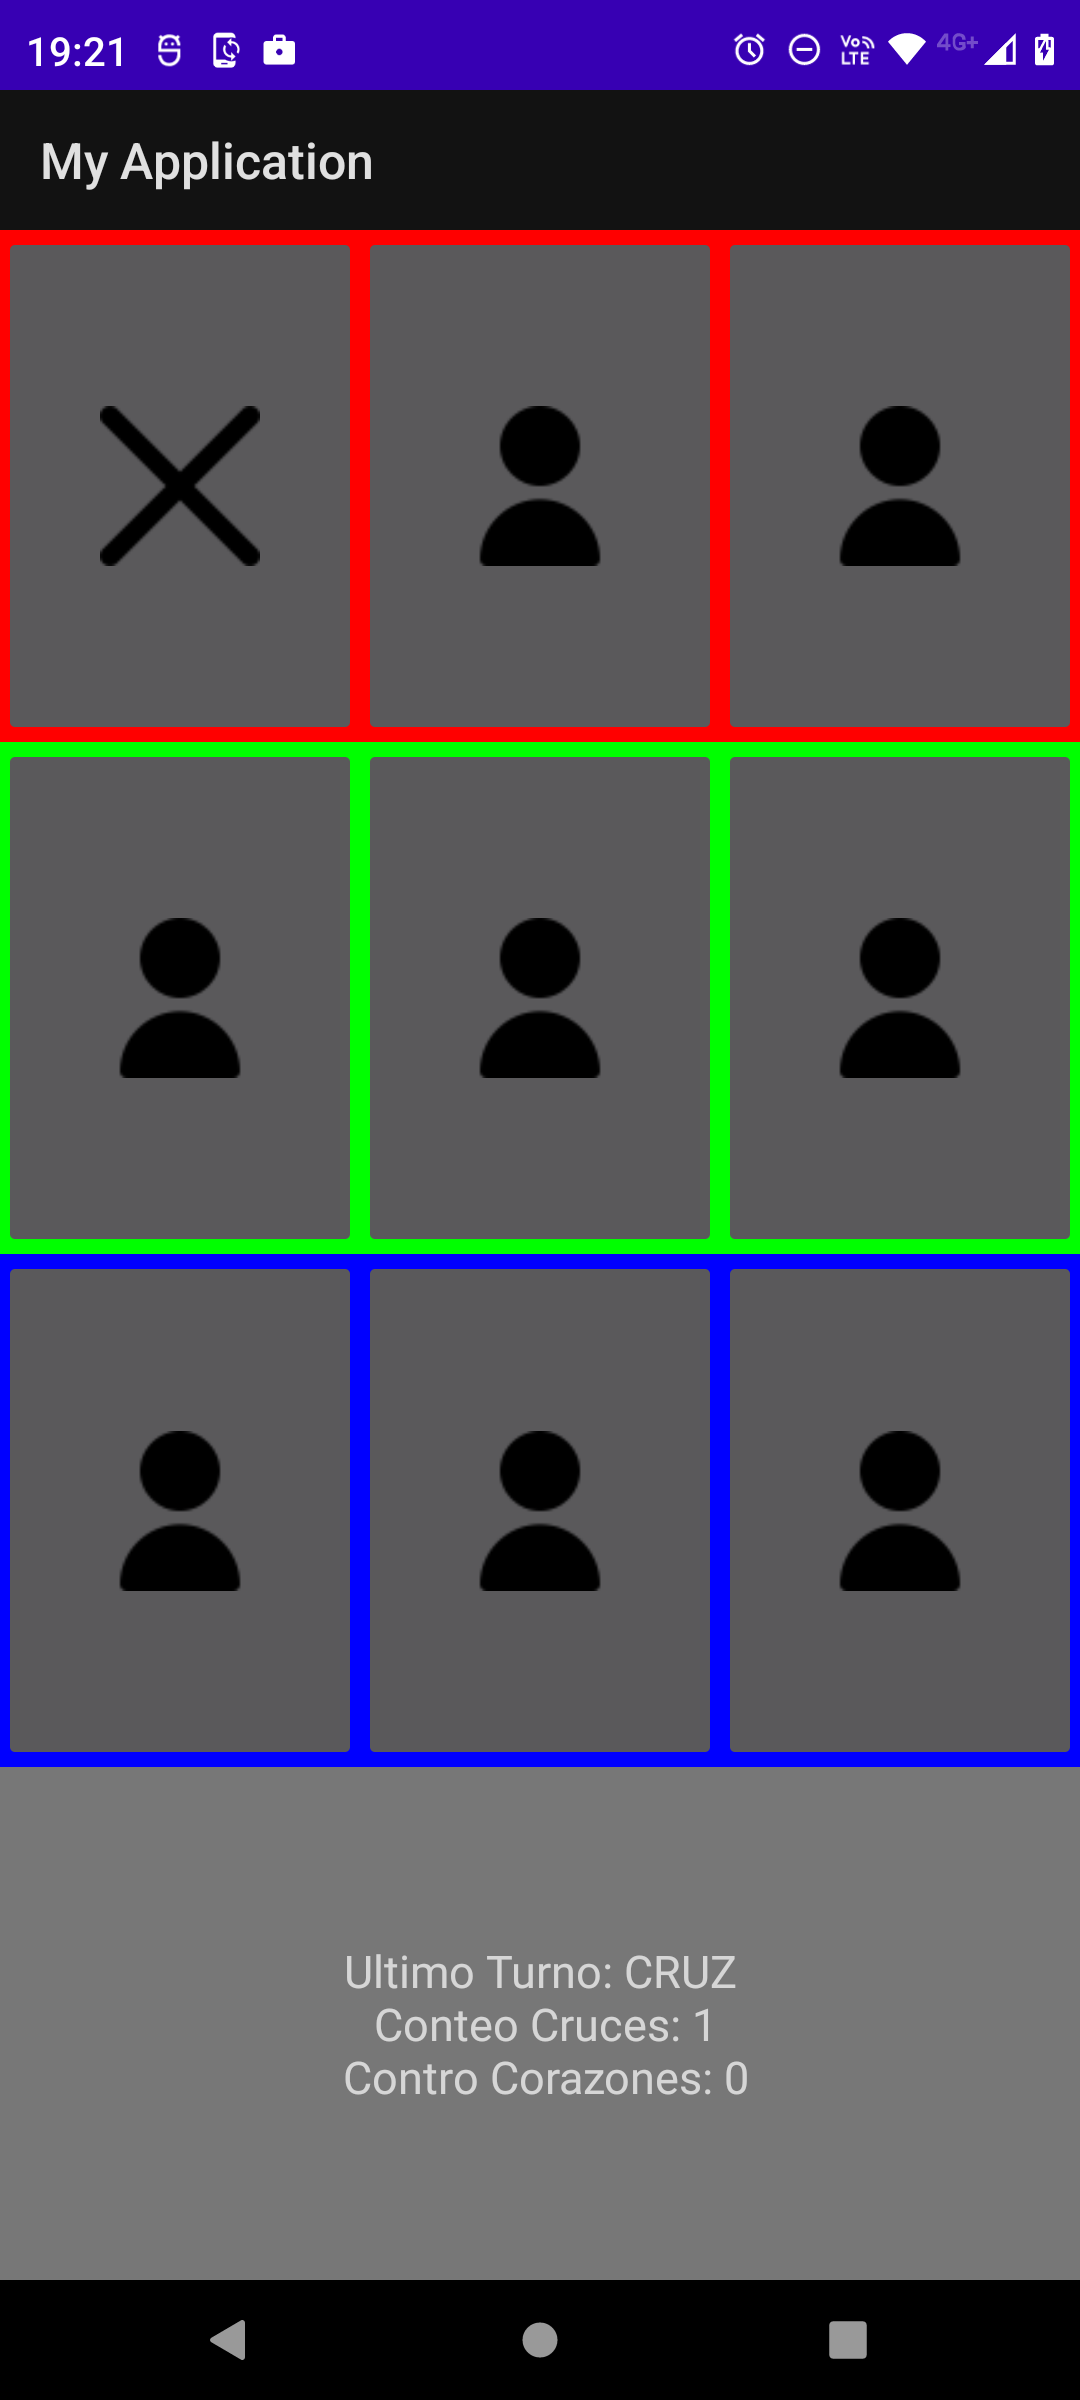
\includegraphics[width=0.95\linewidth]{00_ComportamientoAplicacionTicTacToe/Etapa2_Fase2A.png}    
\end{center}
\column{0.20\linewidth}
\begin{center}
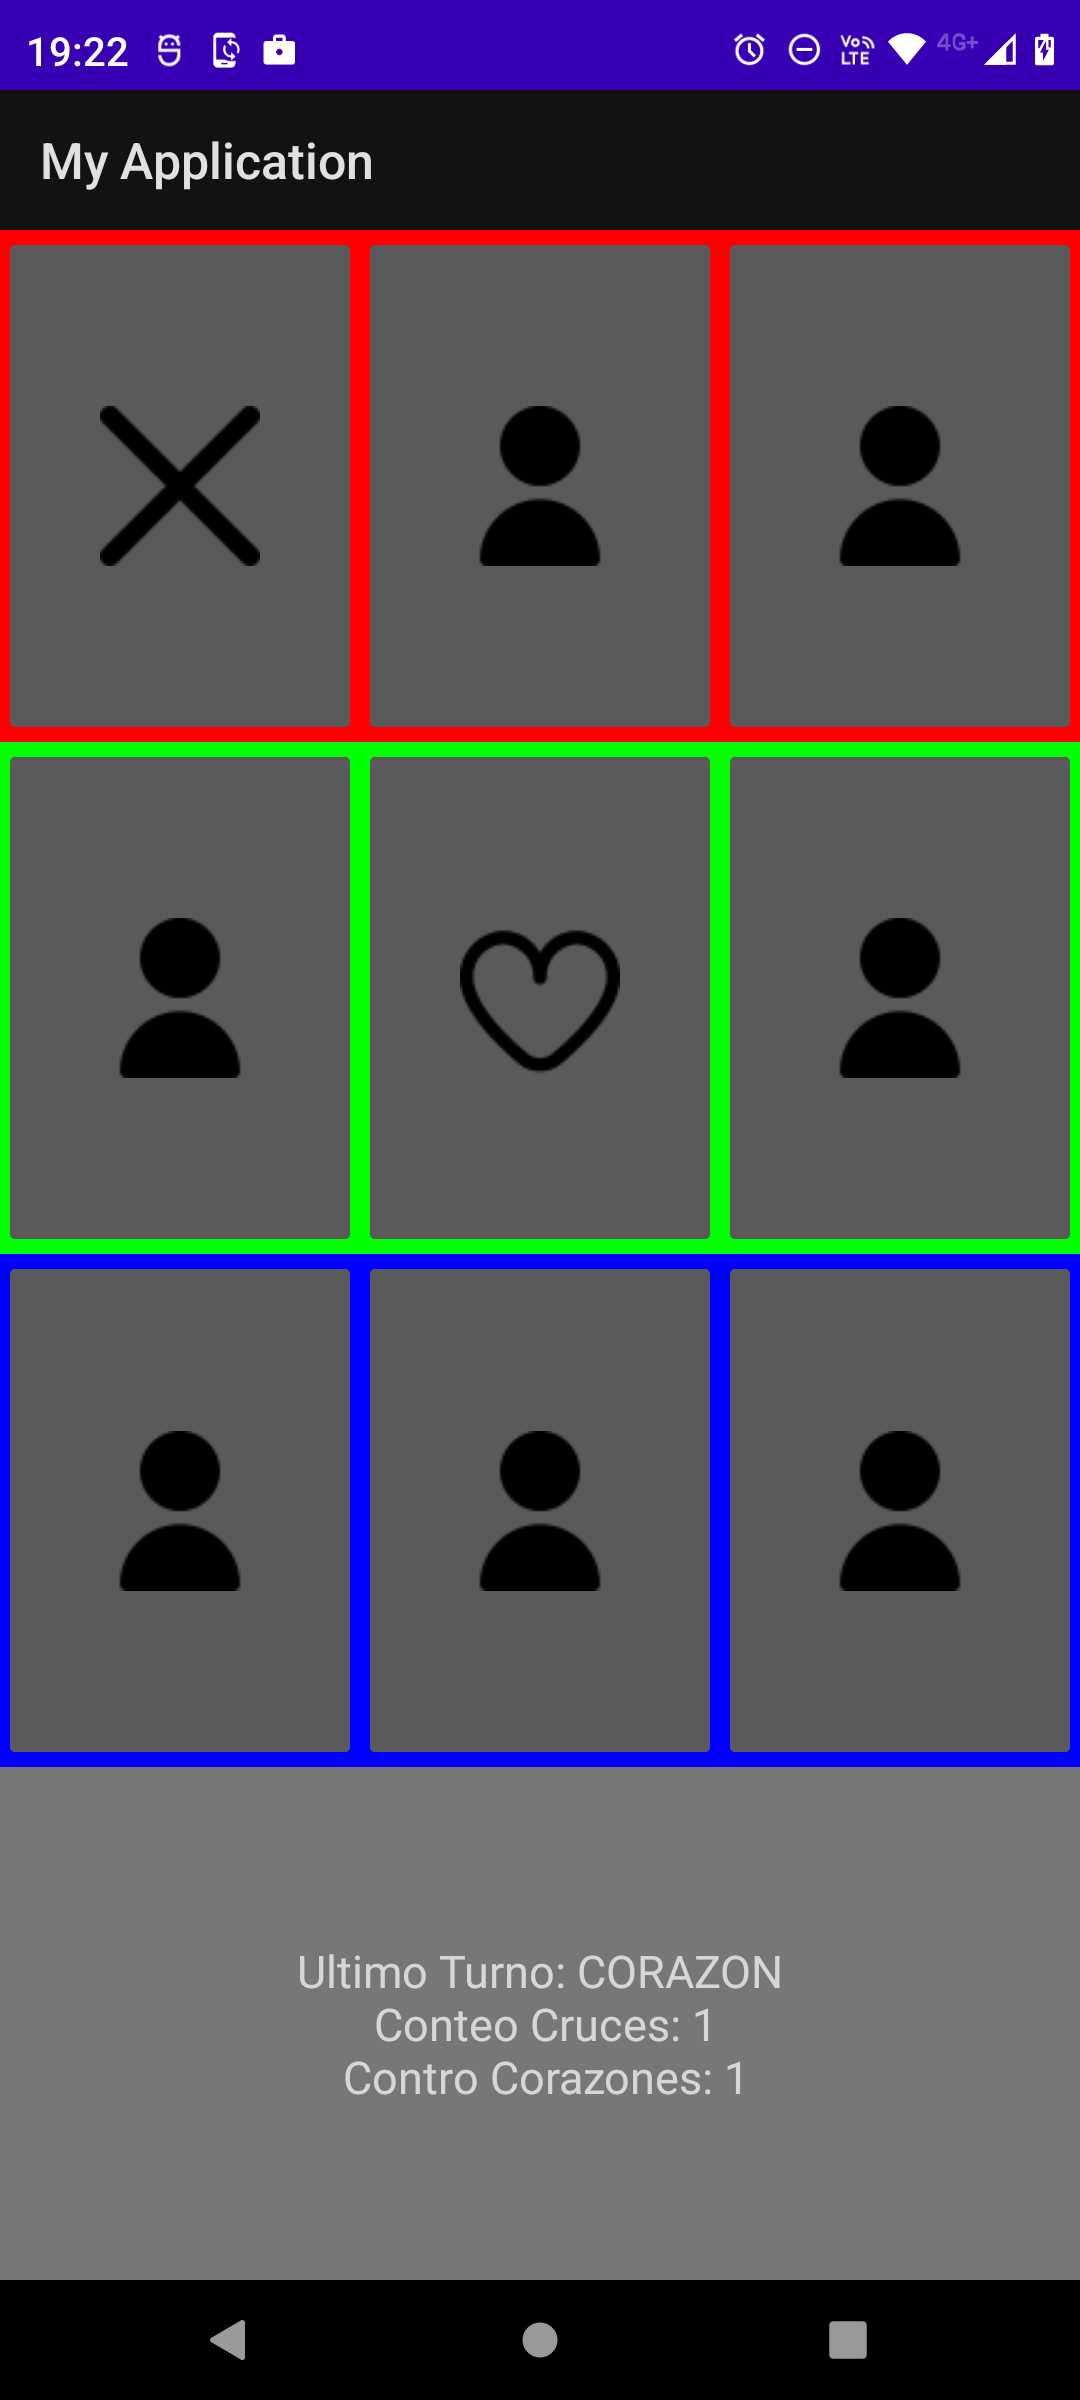
\includegraphics[width=0.95\linewidth]{00_ComportamientoAplicacionTicTacToe/Etapa2_Fase2B.png}    
\end{center}

\end{columns}
\end{frame}



\begin{frame}[fragile]
\frametitle{Problemas pendientes de resolver} 
\begin{columns}
\column{0.58\linewidth}
\begin{enumerate}
\item No detecta al ganador
\item Permite continuar el juego aun habiendo ganado uno (o dos)
\item No detecta el empate
\end{enumerate}

\column{0.20\linewidth}
\begin{center}
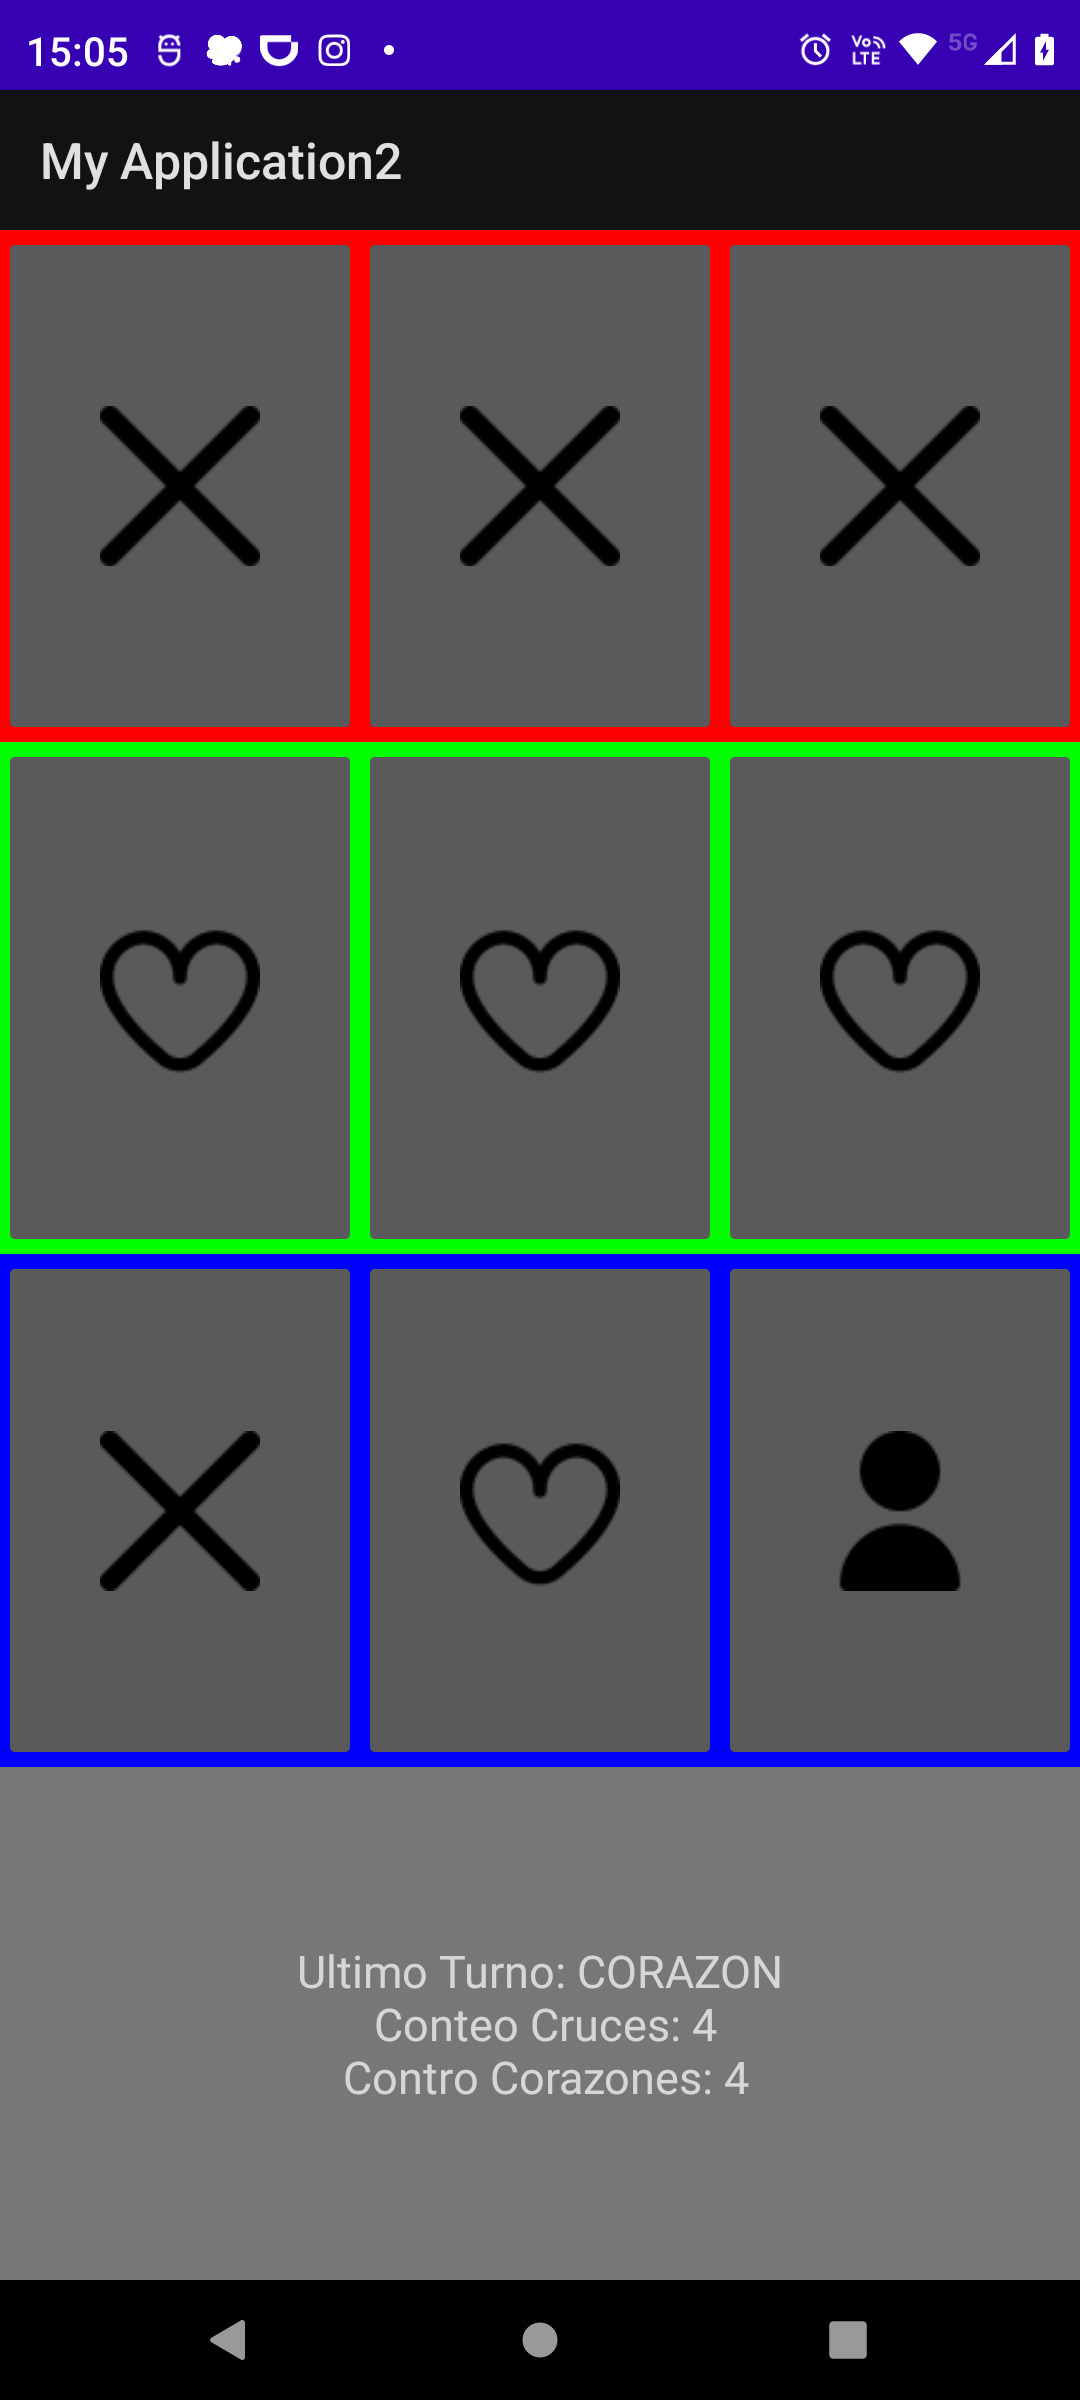
\includegraphics[width=0.95\linewidth]{00_ComportamientoAplicacionTicTacToe/Etapa2_Fase2C.png}  
\end{center}

\column{0.20\linewidth}
\begin{center}
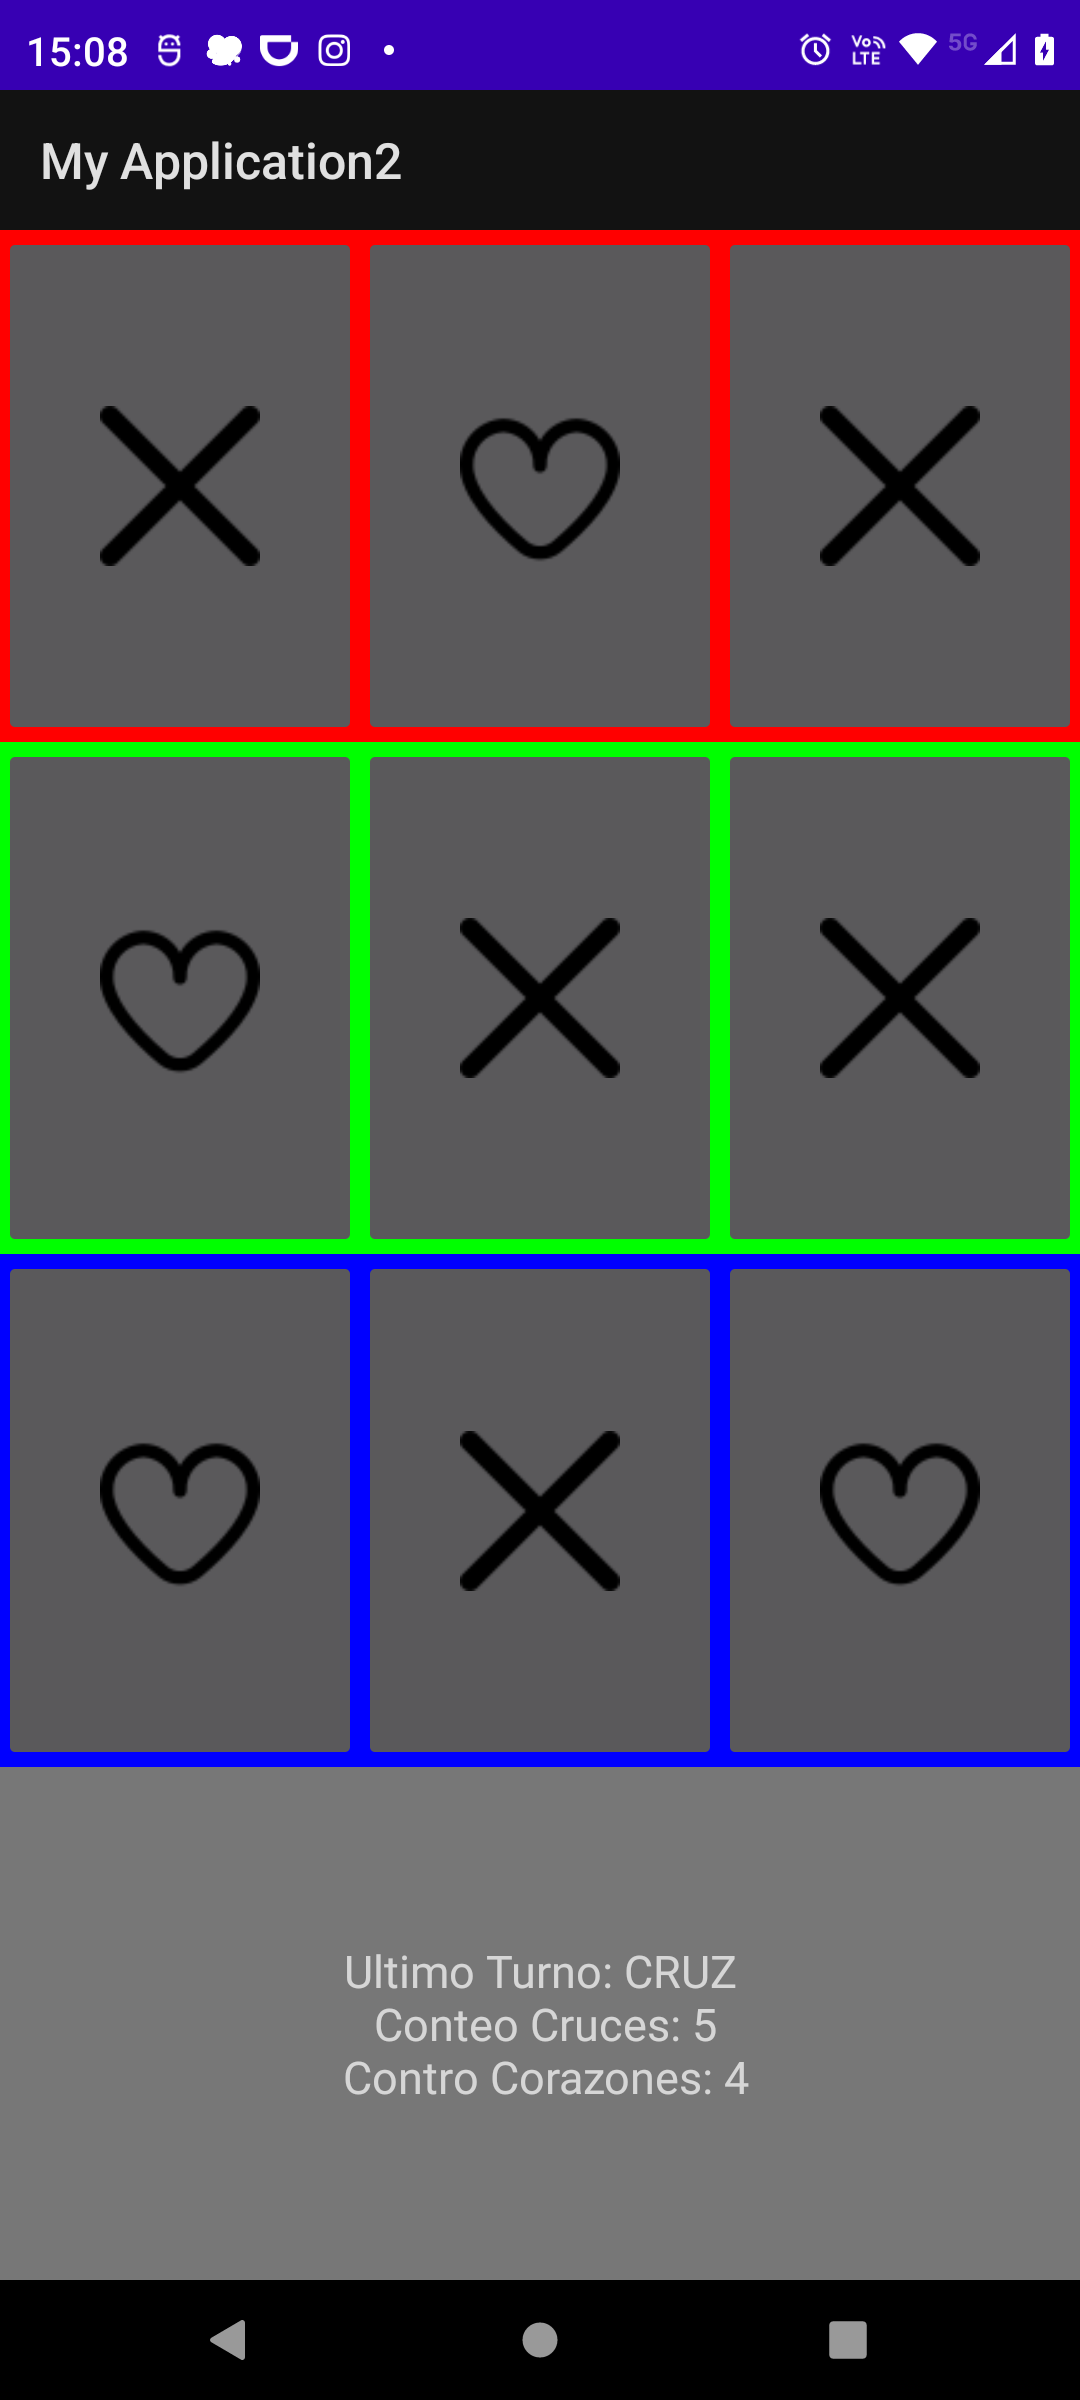
\includegraphics[width=0.95\linewidth]{00_ComportamientoAplicacionTicTacToe/Etapa2_Fase2D.png}  
\end{center}
\end{columns}
\end{frame}


\begin{frame}[fragile]
\frametitle{Fase 3: Checar Ganador (1)} 
\begin{columns}
\column{0.95\linewidth}
\begin{block}{(*4)}
\inputminted[linenos,fontsize=\tiny]{kotlin}{00_ComportamientoAplicacionTicTacToe/MostrarAlertDialog.kt}
\end{block}
\column{0.04\linewidth}
\end{columns}
\end{frame}

\begin{frame}[fragile]
\frametitle{Fase 3: Checar Ganador (2)} 
\begin{columns}
\column{0.95\linewidth}
\begin{block}{(*4)}
\inputminted[linenos,fontsize=\tiny]{kotlin}{00_ComportamientoAplicacionTicTacToe/ChecarGanadorPorFilas.kt}
\end{block}
\column{0.04\linewidth}
\end{columns}
\end{frame}

\begin{frame}[fragile]
\frametitle{Fase 3: Checar Ganador (3)} 
\begin{columns}
\column{0.95\linewidth}
\begin{block}{(*4)}
\inputminted[linenos,fontsize=\tiny]{kotlin}{00_ComportamientoAplicacionTicTacToe/ChecarGanadorPorColumnas.kt}
\end{block}
\column{0.04\linewidth}
\end{columns}
\end{frame}


\begin{frame}[fragile]
\frametitle{Fase 3: Checar Ganador (4)} 
\begin{columns}
\column{0.95\linewidth}
\begin{block}{(*4)}
\inputminted[linenos,fontsize=\tiny]{kotlin}{00_ComportamientoAplicacionTicTacToe/ChecarGanadorPorDiagonales.kt}
\end{block}
\column{0.04\linewidth}
\end{columns}
\end{frame}

\begin{frame}[fragile]
\frametitle{Fase 3: Checar Ganador (5)} 
\begin{columns}
\column{0.95\linewidth}
\begin{block}{(*4)}
\inputminted[linenos,fontsize=\tiny]{kotlin}{00_ComportamientoAplicacionTicTacToe/ChecarAlgunGanadorFin.kt}
\end{block}
\column{0.04\linewidth}
\end{columns}
\end{frame}

\begin{frame}[fragile]
\frametitle{Fase 3: Checar Ganador (6)} 
\begin{columns}
\column{0.58\linewidth}
\begin{block}{(*4) - Actualizar}
\inputminted[linenos,fontsize=\tiny]{kotlin}{00_ComportamientoAplicacionTicTacToe/listenerVersion2.kt}
\end{block}

\begin{block}{}
¿Qu\'e problema falta por resolverse?
\end{block}

\column{0.20\linewidth}
\begin{center}
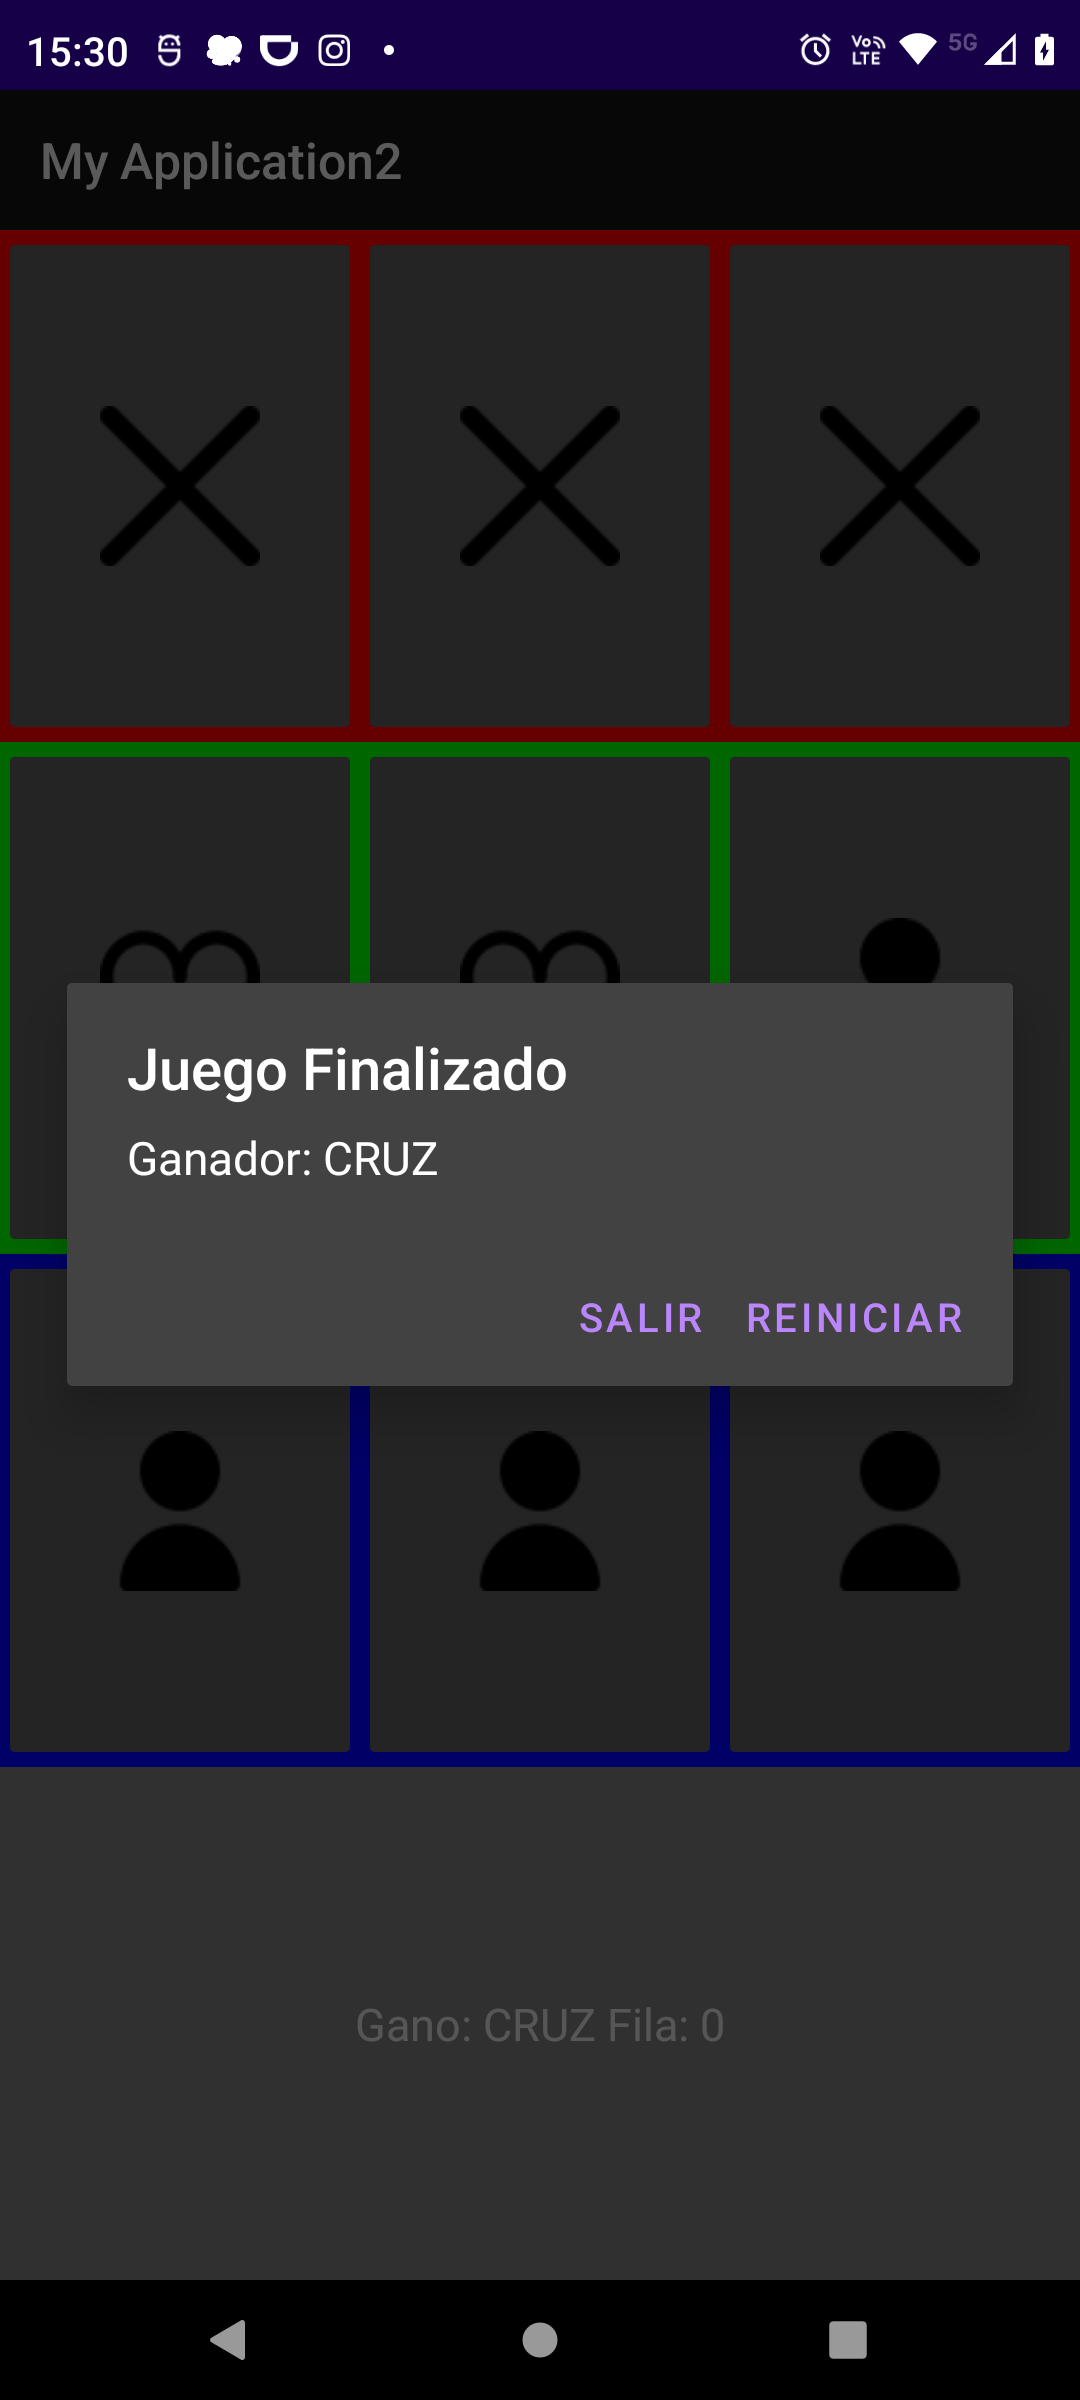
\includegraphics[width=0.95\linewidth]{00_ComportamientoAplicacionTicTacToe/Etapa3_Fase1A.png}  
\end{center}
\column{0.20\linewidth}
\begin{center}
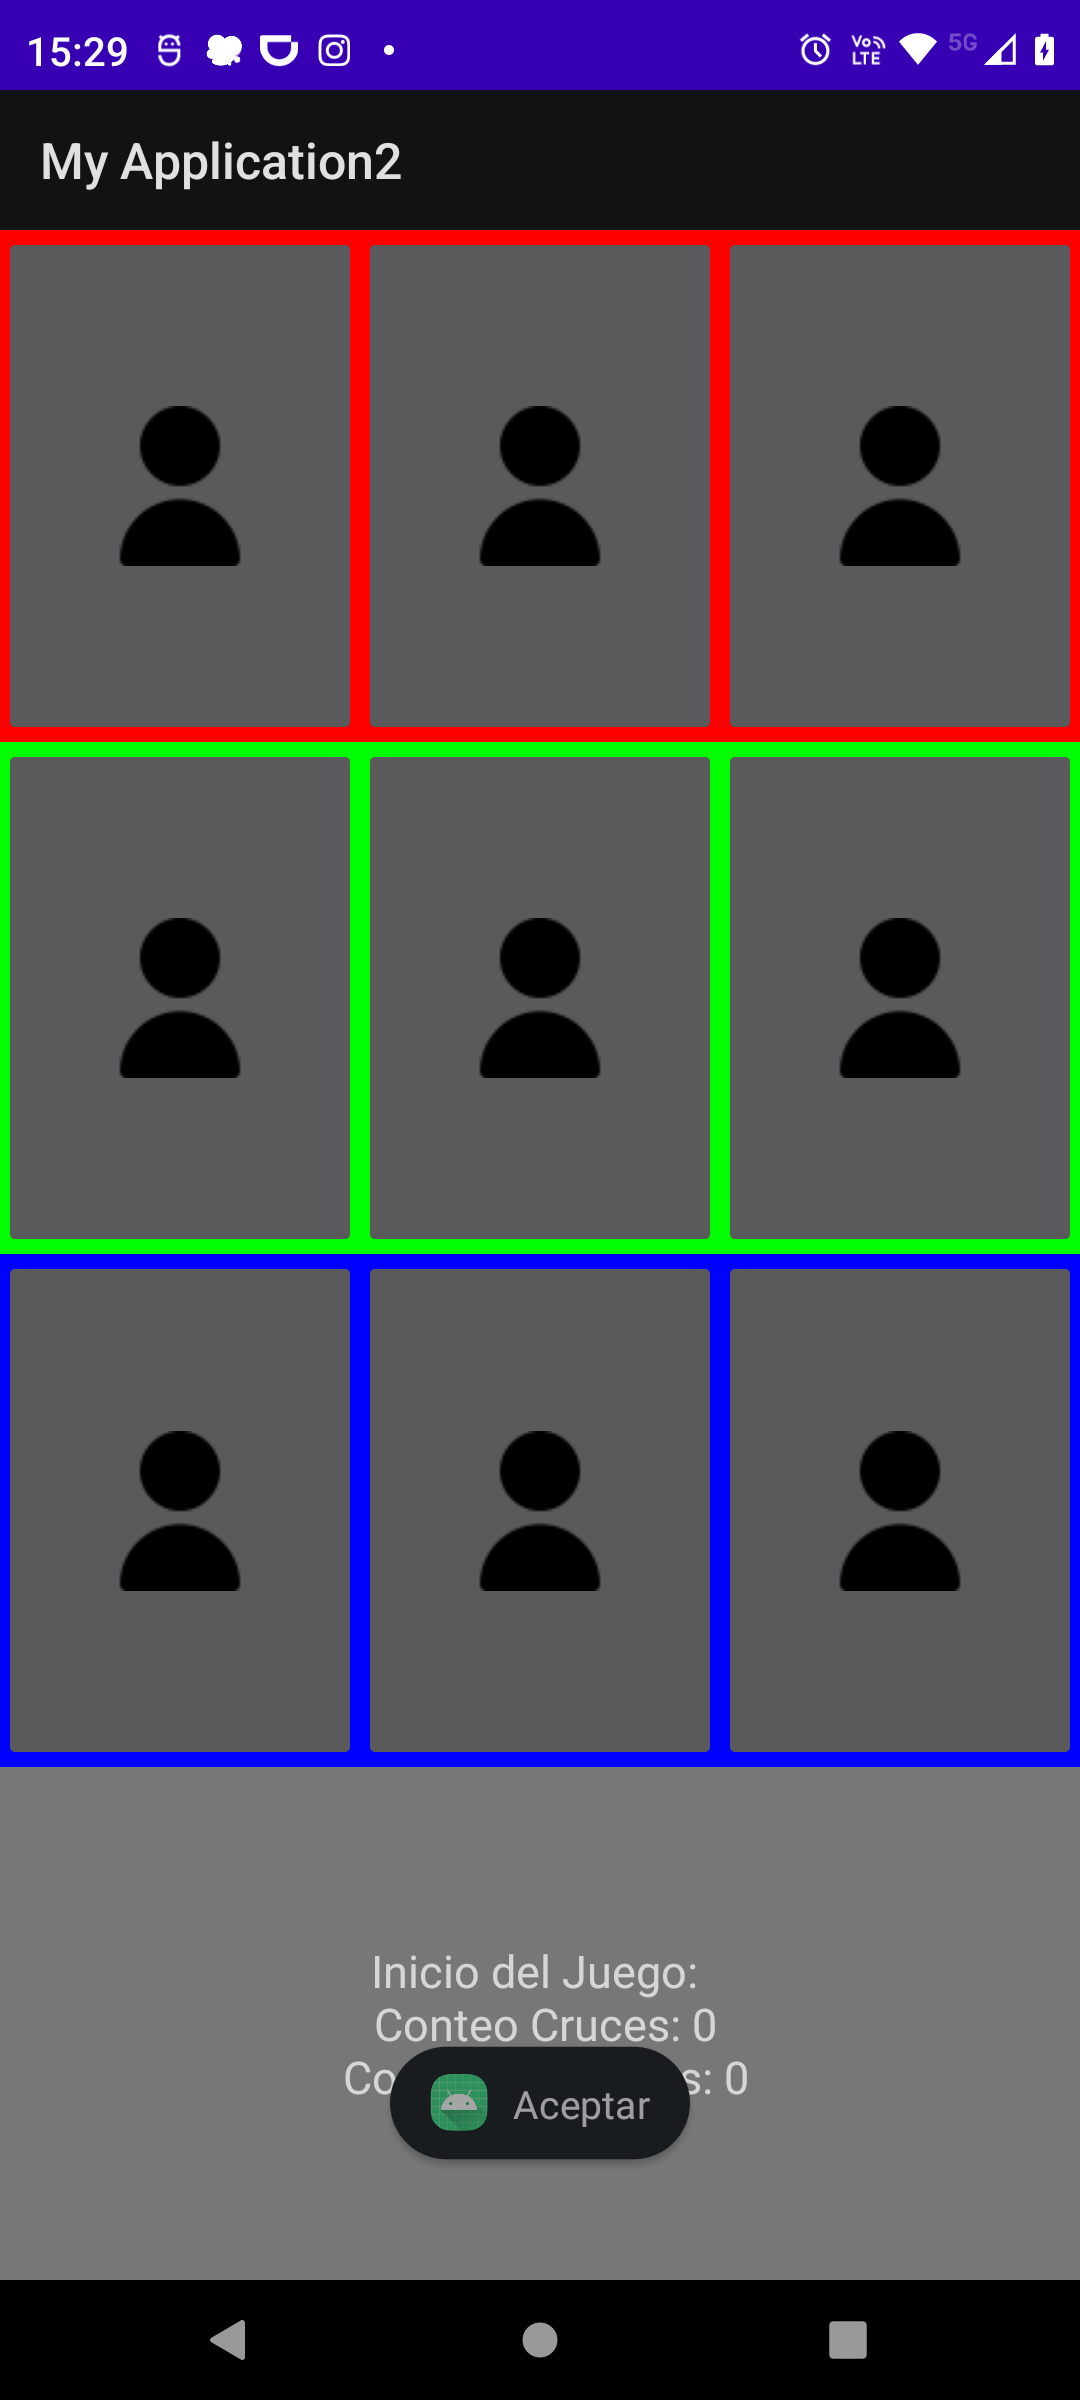
\includegraphics[width=0.95\linewidth]{00_ComportamientoAplicacionTicTacToe/Etapa3_Fase1B.png}  
\end{center}
\end{columns}
\end{frame}

\begin{frame}[fragile]
\frametitle{Fase 4: Checar Empate} 
\begin{columns}
\column{0.58\linewidth}
\begin{block}{(*4)}
\inputminted[linenos,fontsize=\tiny]{kotlin}{00_ComportamientoAplicacionTicTacToe/ChecarEmpate.kt}
\end{block}

\begin{block}{(*4) - Actualizar}
\inputminted[linenos,fontsize=\tiny]{kotlin}{00_ComportamientoAplicacionTicTacToe/listenerVersion3.kt}
\end{block}
\column{0.20\linewidth}
\begin{center}
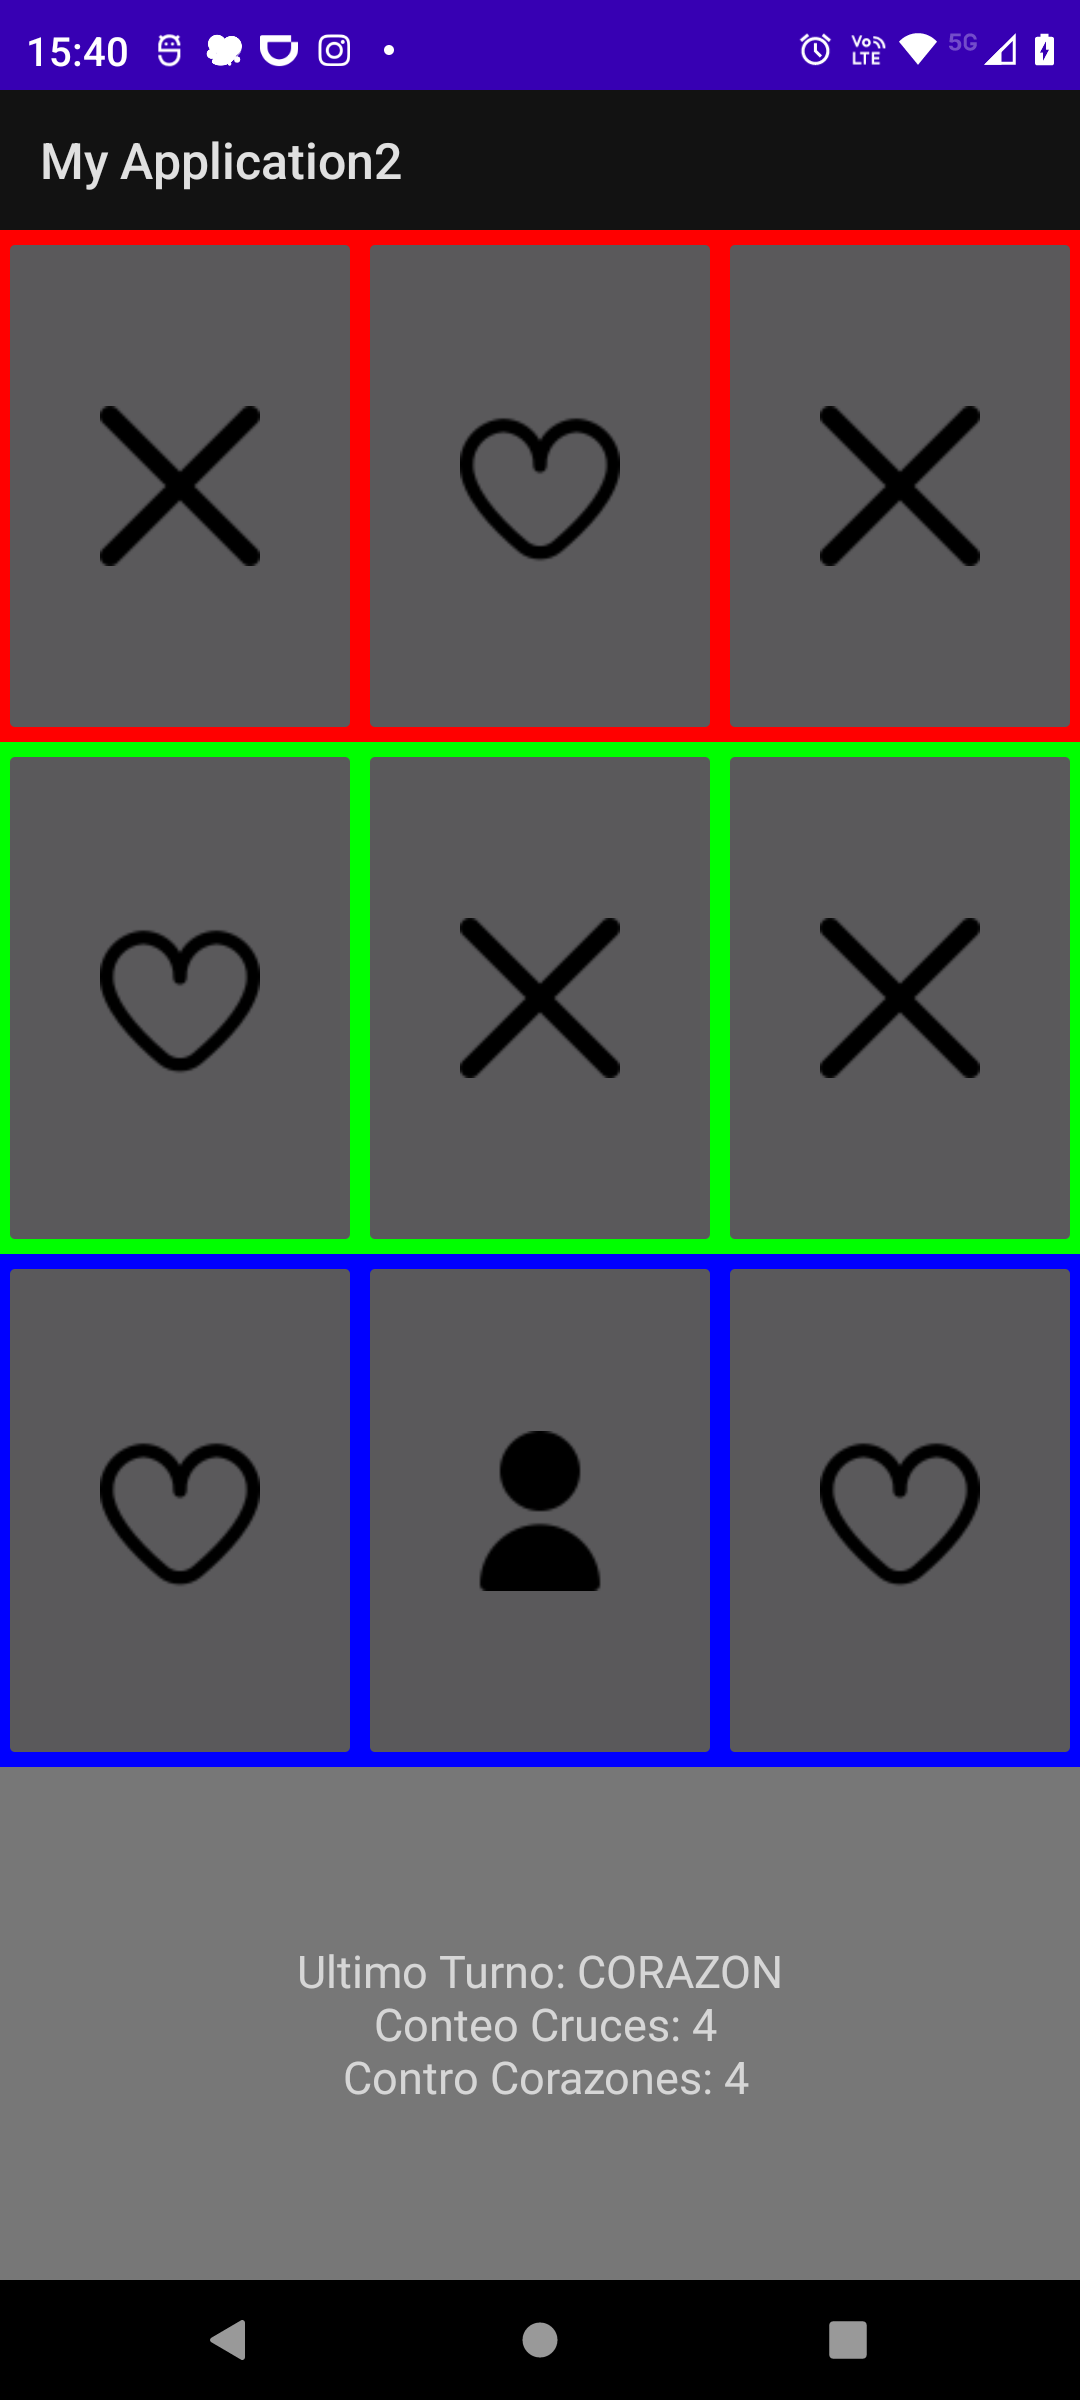
\includegraphics[width=0.95\linewidth]{00_ComportamientoAplicacionTicTacToe/Etapa3_Fase2A.png}  
\end{center}
\column{0.20\linewidth}
\begin{center}
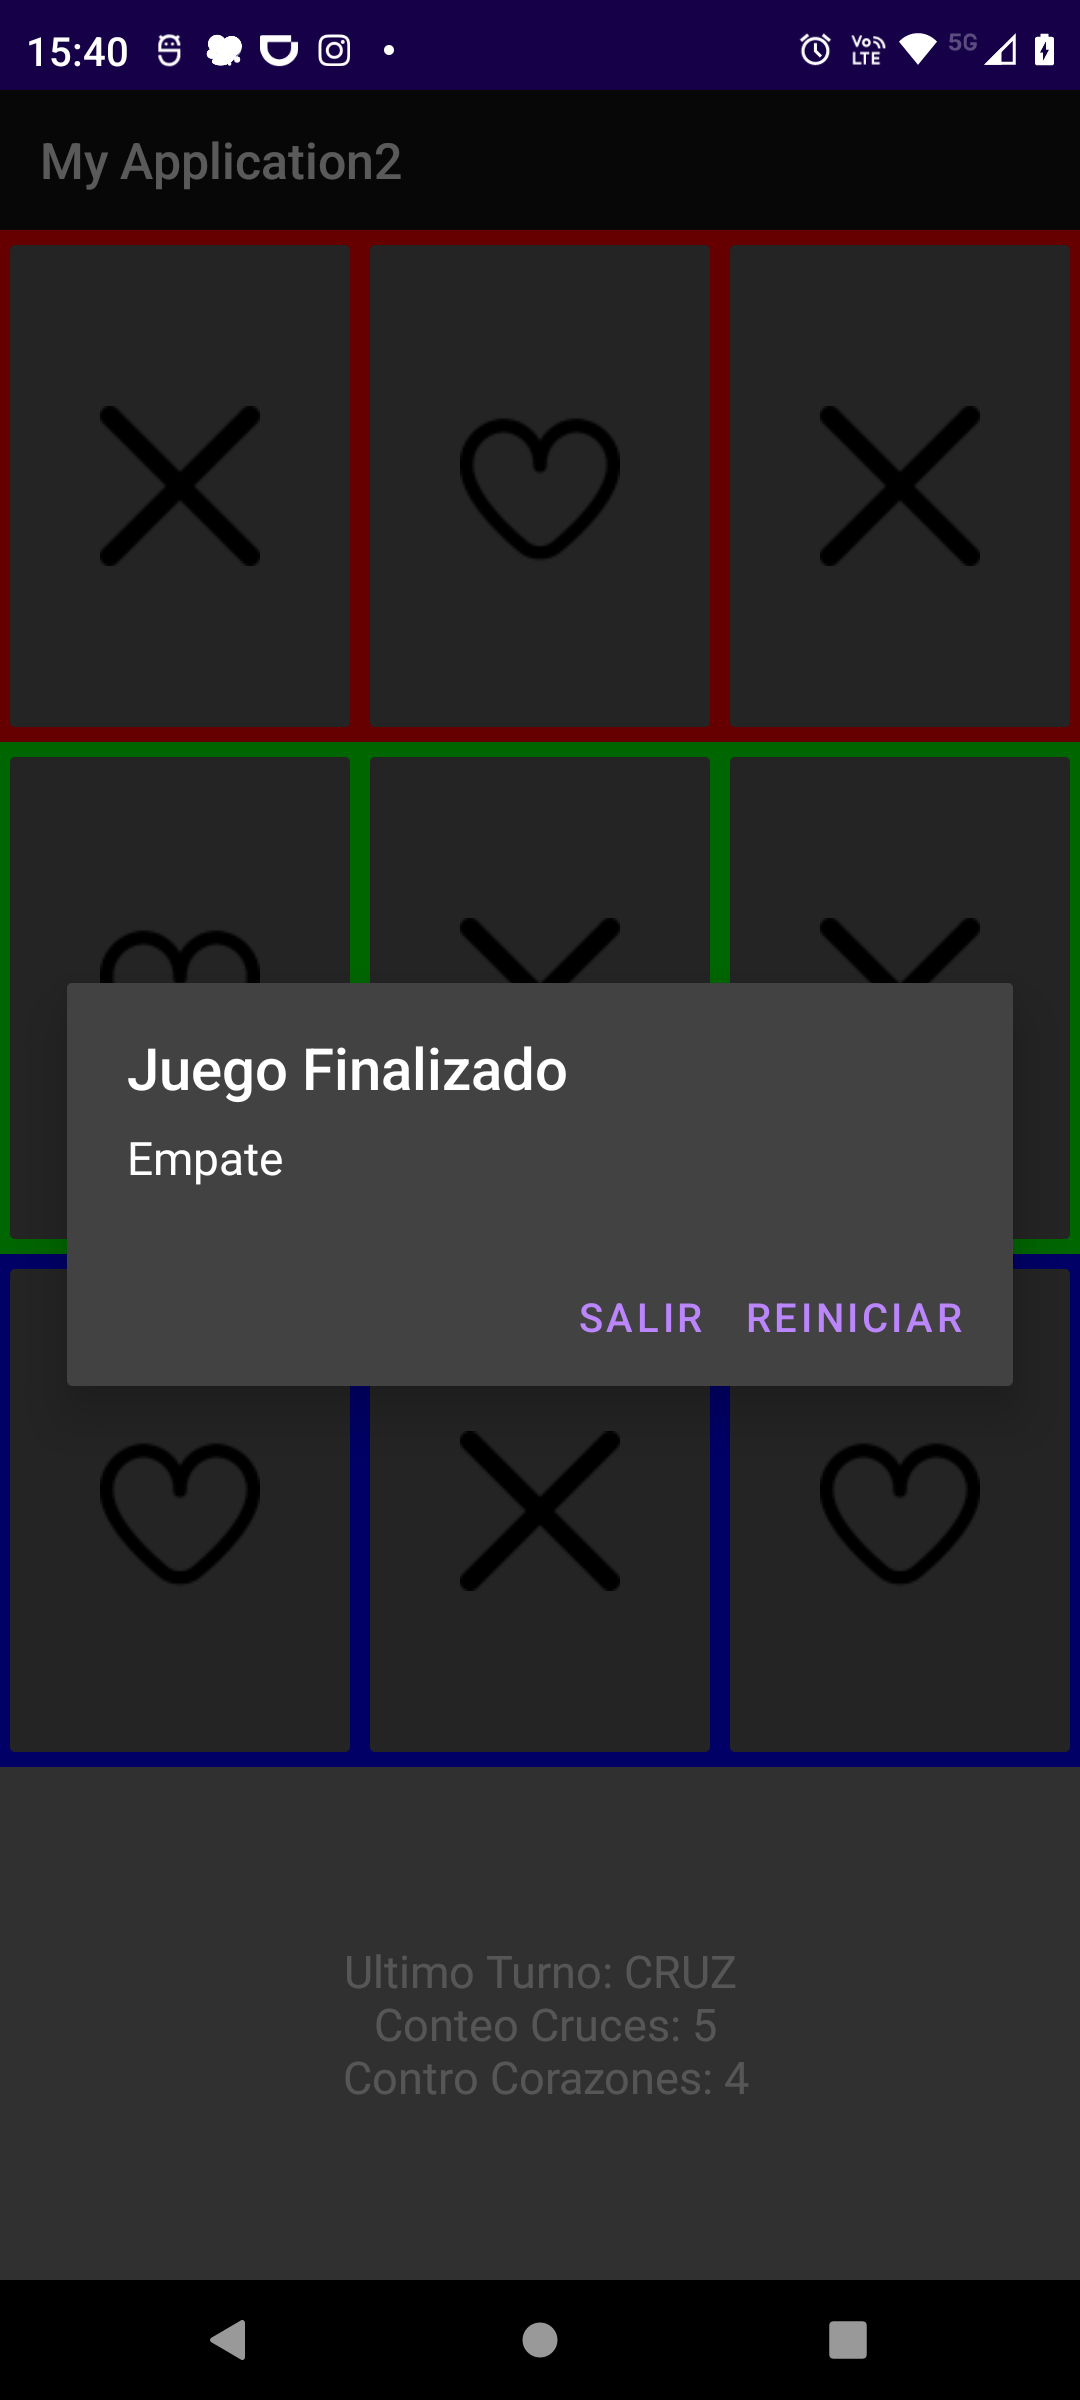
\includegraphics[width=0.95\linewidth]{00_ComportamientoAplicacionTicTacToe/Etapa3_Fase2B.png}  
\end{center}
\end{columns}
\end{frame}

